\documentclass[11pt]{article}
\usepackage[a4paper,margin=26mm]{geometry}
\usepackage[T1]{fontenc}
\usepackage{lmodern,microtype}
\usepackage{amsmath,amssymb,amsthm,mathtools}
\usepackage{booktabs,tabularx,array,graphicx,xcolor,enumitem}
\usepackage{fancyhdr}
\usepackage[colorlinks=true,linkcolor=blue!45!black,citecolor=blue!45!black,urlcolor=blue!45!black]{hyperref}
\hypersetup{pdftitle={A sharp 25/27 threshold for cubic Euler-factor agreement},pdfauthor={Research prepared for Vladimir Reshetnikov}}
\setlength{\headheight}{14pt}
\pagestyle{fancy}\fancyhf{}\fancyhead[L]{\small Cubic Euler-factor agreement}\fancyhead[R]{\small 27 November 2026}\fancyfoot[C]{\thepage}
\setlength{\parskip}{4pt}\setlength{\parindent}{0pt}
\setlist{nosep,leftmargin=*}
\newtheorem{theorem}{Theorem}[section]
\newtheorem{proposition}[theorem]{Proposition}
\newtheorem{lemma}[theorem]{Lemma}
\newtheorem{corollary}[theorem]{Corollary}
\theoremstyle{definition}\newtheorem{definition}[theorem]{Definition}
\theoremstyle{remark}\newtheorem{remark}[theorem]{Remark}
\newcommand{\C}{\mathbb C}\newcommand{\Q}{\mathbb Q}\newcommand{\F}{\mathbb F}\newcommand{\Z}{\mathbb Z}
\newcommand{\T}{\mathbb T}\newcommand{\E}{\mathbb E}\newcommand{\GL}{\mathrm{GL}}\newcommand{\SU}{\mathrm{SU}}\newcommand{\U}{\mathrm U}
\newcommand{\tr}{\operatorname{tr}}\newcommand{\Gal}{\operatorname{Gal}}\newcommand{\diag}{\operatorname{diag}}
\newcommand{\scal}{\mathrm{sc}}\newcommand{\dist}{\operatorname{dist}}\newcommand{\id}{\mathrm{id}}
\newcommand{\abs}[1]{\left|#1\right|}\newcommand{\norm}[1]{\left\|#1\right\|}
\newcommand{\repo}{https://github.com/VladimirReshetnikov/ProveIt}
\newcommand{\commit}{8528159d15e864e603ba4ded6ebb694c48cf160b}
\newcommand{\repobase}{https://github.com/VladimirReshetnikov/ProveIt/blob/8528159d15e864e603ba4ded6ebb694c48cf160b/Analysis/GeneralizedRiemannHypothesis}
\newcommand{\pathcode}[1]{\texttt{\detokenize{#1}}}
\title{\textbf{A sharp \texorpdfstring{$25/27$}{25/27} threshold\\for cubic Euler-factor agreement}\\[5pt]\large Rigidity, reducibility, stability, and a tempered \texorpdfstring{$\GL_3$}{GL3} theorem}
\author{Research manuscript prepared for Vladimir Reshetnikov}
\date{27 November 2026}
\begin{document}
\maketitle
\begin{abstract}
For any two inequivalent continuous three-dimensional complex representations of a compact group, the complete characteristic polynomials disagree on Haar measure at least $2/27$. This constant is exact, including for irreducible finite-image Artin representations. We classify every equality case: both representations are irreducible, their determinants agree, and they have the same scalar kernel of index nine, with projective quotient $C_3\times C_3$. If either representation is reducible, the exact universal lower bound improves to $1/8$. Near the $2/27$ threshold, a quantitative inequality forces the matrices on the disagreement set to be nearly scalar. The threshold also gives optimal universal erasure and corruption bounds for complete local factors. We give explicit order-$27$ matrices and an explicit Galois extension of $\Q(\sqrt{-3})$ realizing equality.

The same determinant argument, combined with the standard Rankin--Selberg second moment, proves the sharp lower Dirichlet density $2/27$ for complete-factor disagreement of distinct tempered unitary cuspidal representations of $\GL_3$. Temperedness remains an assumption for general automorphic representations. The construction extends the repository's Euler-factor support methods to nonabelian irreducible factors; the finite and compact group results do not require RH or GRH. Targeted searches found no prior statement of this exact full-factor theorem, but publication priority is not certified.
\end{abstract}

\section{Outcome, source framework, and status}

The decisive observation is that a cubic Euler factor records a determinant as well as a trace. If two determinant characters are different, at least half the group already distinguishes them. If they agree, the two traces, after a common pointwise normalization, lie in an equilateral triangle of diameter $3\sqrt3$. Orthogonality then forces disagreement on at least $2/27$ of the group. A Heisenberg group attains the bound.

This is an exact extremal result in the refined strong-multiplicity-one program. It is not a proof of the general trace-density conjecture or of generalized Ramanujan. The distinction between trace data and full local factors matters even in the smallest sharp examples. A separate companion note, \emph{Counterexamples to Rajan's Euler-factor agreement conjecture}, uses the repository's abelian cubic packets to disprove Conjecture~3 of \cite{Rajan2000} as stated. That abelian conjecture is distinct from the cuspidal trace-density problem discussed here.

\subsection{What was analyzed in ProveIt}

The source snapshot is commit
\href{\repo/commit/\commit}{\texttt{8528159d15e}} of
\pathcode{Analysis/GeneralizedRiemannHypothesis/}. Its inventory lists 194 merged reports and 15 additional research packets. We inspected the exported Lean statements, the source-method section, the relevant matching, nonabelian, analytic and geometric sections, and the additional packet inventory. This was a targeted mathematical audit, not independent verification of all 194 reports and not a fresh Lean-kernel replay.

\begin{center}\small
\begin{tabularx}{\linewidth}{@{}>{\raggedright\arraybackslash}p{.30\linewidth}>{\raggedright\arraybackslash}X@{}}\toprule
Repository component & Role in the present work\\\midrule
Vendor files \pathcode{Statements.lean} and \pathcode{Main.lean} & Export RH and nonvanishing/critical-line statements for Dirichlet $L$-functions. They do not export general Artin GRH, zero simplicity or generalized Ramanujan.\\
\pathcode{rec.tex}, labels \pathcode{rec:sec:qmatch}, \pathcode{rec:sec:omatch} & Treat agreement of Euler factors of products of one-dimensional characters by converting agreement into small support.\\
\pathcode{nab.tex} & Develops nonabelian character detectors and makes the missing arithmetic estimates explicit.\\
\pathcode{gra.tex}, label \pathcode{gra:sec:ehrhart} & Gives a finite-width canonical-line/interlacing theorem. An attempted uniform extension here did not close its positivity gap.\\\bottomrule
\end{tabularx}
\end{center}

The transfer is methodological: retain a nonnegative quantity with a known global average, exploit its vanishing on the agreement set, and determine its sharp local maximum. Here that quantity is a squared character difference. The new ingredient is the determinant constraint on cubic unitary traces, followed by exact equality and stability analysis.

\subsection{Proof and novelty labels}

The group-theoretic results below have complete proofs. The arithmetic corollaries use the classical Chebotarev theorem. The automorphic extension uses established Rankin--Selberg analytic properties and cyclic automorphic induction, with references below. The exact finite checks supplement these proofs. No new Lean theorem or formal verification of the manuscript is claimed.

The closest literature we located is Martin--Walji's study of \emph{trace} disagreement and primitive finite-group characters \cite{MartinWalji}, Rajan's density refinements \cite{Rajan2000,Rajan2003}, and Walji's formulation of the trace-density conjecture \cite{Walji}. The exact $25/27$ complete-factor threshold, its equality classification, the sharp reducibility gap and the stability statement were not found in the inspected repository material or targeted searches. This is a provisional novelty assessment, not a claim that all literature has been exhausted.

\section{Definitions and main theorem}

Let $G$ be a compact Hausdorff group with normalized Haar probability measure $m$. All representations are continuous, finite dimensional, and complex. Averaging a Hermitian inner product makes them unitary; characteristic polynomials are unchanged. Finite groups are included with $m(A)=|A|/|G|$.

For a representation $\rho:G\to\U(3)$ define
\[
 P_\rho(g,T)=\det(I-T\rho(g)),\qquad \chi_\rho(g)=\tr\rho(g),\qquad d_\rho(g)=\det\rho(g).
\]
The polynomial $P_\rho$ is the reciprocal Euler-factor polynomial. Equality of these polynomials is equivalent to equality of $\det(TI-\rho(g))$.

\begin{definition}
The full-factor disagreement set and its measure are
\[
 D(\rho,\sigma)=\{g\in G:P_\rho(g,T)\ne P_\sigma(g,T)\},\qquad
 \delta(\rho,\sigma)=m(D(\rho,\sigma)).
\]
The set $D$ is open because the coefficients depend continuously on $g$.
The scalar kernel is the closed normal subgroup
\[
 K_\rho=\{g\in G:\rho(g)\text{ is a scalar matrix}\}.
\]
\end{definition}

\begin{theorem}[Sharp cubic separation and rigidity]\label{thm:main}
Let $\rho,\sigma$ be inequivalent three-dimensional representations of $G$. They need not be irreducible. Then
\begin{equation}\label{eq:main}
 \boxed{\delta(\rho,\sigma)\ge\frac{2}{27}.}
\end{equation}
If $d_\rho\ne d_\sigma$, then $\delta\ge1/2$.

Equality in \eqref{eq:main} holds if and only if both representations are irreducible, their determinant characters agree, and their scalar kernels coincide in an open normal subgroup $K$ of index nine. In this case
\[
 G/K\simeq C_3\times C_3.
\]
Writing $\rho(k)=\lambda(k)I$ and $\sigma(k)=\mu(k)I$ on $K$, the character $\lambda/\mu$ has order three, both traces vanish outside $K$, and
\begin{equation}\label{eq:equalityD}
 D=K\setminus\ker(\lambda/\mu).
\end{equation}
The bound is attained by a group of order $27$.
\end{theorem}

\begin{theorem}[Exact reducibility gap]\label{thm:reducible}
If at least one of the two inequivalent cubic representations is reducible, then
\begin{equation}\label{eq:reducible}
 \boxed{\delta(\rho,\sigma)\ge\frac18.}
\end{equation}
This is sharp for a group of order $16$. Thus a pair with full-factor disagreement below $1/8$ must consist of two irreducible representations.
\end{theorem}

In particular, complete cubic local-factor data form a family whose universal minimum distance is $2/27$, whereas the portion involving reducible representations has minimum distance $1/8$. The hypotheses concern the representations, not the degree of a defining number-field polynomial.

\section{The cubic trace triangle}

Put $\omega=e^{2\pi i/3}$ and
\[
 \Delta=\operatorname{conv}\{3,3\omega,3\omega^2\}\subset\C.
\]

\begin{lemma}[Trace geometry]\label{lem:triangle}
If $U\in\SU(3)$, then $\tr U\in\Delta$. The diameter of $\Delta$ is $3\sqrt3$, and only two distinct vertices attain it. Therefore if $U,V\in\U(3)$ have the same determinant, then
\begin{equation}\label{eq:27}
 |\tr U-\tr V|^2\le27.
\end{equation}
Equality forces $U$ and $V$ to be distinct scalar matrices, and their scalar ratio is a nontrivial cube root of unity.
\end{lemma}

\begin{proof}
Let the eigenvalues of $U\in\SU(3)$ be $a,b,(ab)^{-1}$, with $|a|=|b|=1$. The identity
\begin{equation}\label{eq:triangleidentity}
 3+2\Re\tr U=|1+a+ab|^2\ge0
\end{equation}
is immediate by expansion. Apply it also to $\omega U$ and $\omega^2U$; these matrices still have determinant one. Thus
\[
 \Re(\omega^j\tr U)\ge-\frac32\quad(j=0,1,2).
\]
The intersection of these three half-planes is $\Delta$.

Any difference of two points of $\Delta$ is a convex combination of differences of vertices. Each such difference has modulus at most $3\sqrt3$. If the modulus is maximal, strict convexity of the Euclidean disk forces every nonzero-weight vertex difference to be the same diameter vector. Its ordered pair of vertices is unique; hence the original points are these two vertices.

For equal determinants choose any $\alpha\in\T$ with $\alpha^3=\det U=\det V$. Then $\alpha^{-1}U,\alpha^{-1}V\in\SU(3)$, giving \eqref{eq:27}. This choice is made separately at each group element; no cube-root character is assumed. A unitary matrix whose trace has modulus three has all eigenvalues equal, by equality in the triangle inequality. The equality assertion follows.
\end{proof}

\begin{figure}[ht]
\centering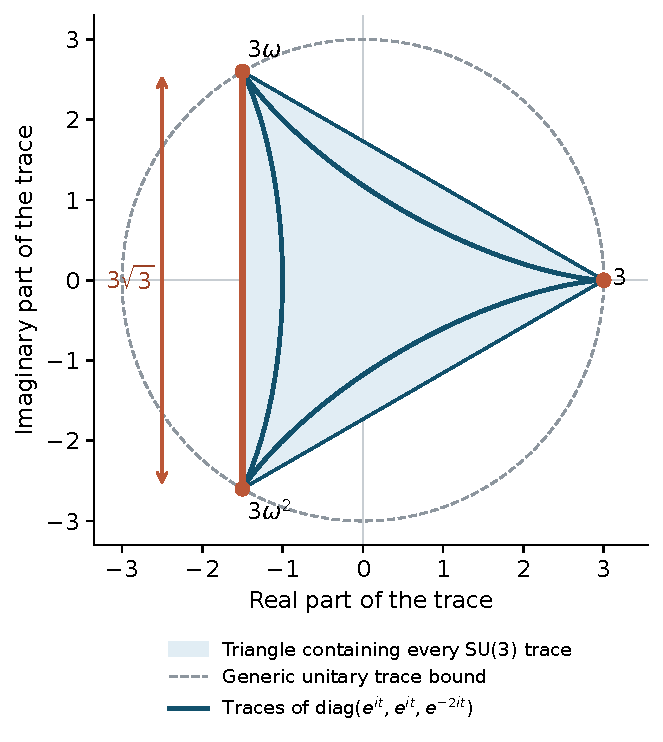
\includegraphics[width=.77\linewidth]{figures/trace_triangle.pdf}
\caption{The determinant-one trace triangle has squared diameter $27$. The generic radius-three disk only gives squared diameter $36$. The curved trace locus is illustrative; the proof uses the elementary identity \eqref{eq:triangleidentity}, not a numerical description of that locus.}
\label{fig:triangle}
\end{figure}

\begin{lemma}[A cubic unitary polynomial]\label{lem:poly}
For $U\in\U(3)$, put $z=\tr U$ and $d=\det U$. Then
\begin{equation}\label{eq:poly}
 \det(I-TU)=1-zT+d\overline z\,T^2-dT^3.
\end{equation}
Consequently, for two unitary cubic matrices with equal determinant, equality of traces is equivalent to equality of the complete characteristic polynomials.
\end{lemma}

\begin{proof}
If the eigenvalues are $u_1,u_2,u_3$, their second elementary symmetric function is
$d(u_1^{-1}+u_2^{-1}+u_3^{-1})=d\overline z$, since $|u_i|=1$.
\end{proof}

\section{Separation and the sharp equality cases}

\subsection{The determinant dichotomy}

The quotient $\eta=d_\rho/d_\sigma:G\to\T$ is a continuous one-dimensional character. If it is nontrivial, its compact image is either cyclic of order $r\ge2$ or all of $\T$. Haar measure pushes forward to normalized Haar measure on that image. Therefore
\[
 m(\ker\eta)=1/r\le1/2\quad\hbox{or}\quad m(\ker\eta)=0.
\]
Since $G\setminus\ker\eta\subset D$, we obtain $\delta\ge1/2$. Hence any pair close to the extremal $2/27$ threshold automatically has equal determinant characters.

\subsection{Character energy, including reducible representations}

Write the finite irreducible decompositions
\[
 \rho\simeq\bigoplus_\tau m_\tau\tau,\qquad
 \sigma\simeq\bigoplus_\tau n_\tau\tau.
\]
Orthogonality of irreducible characters gives the integer
\begin{equation}\label{eq:energy}
 M:=\int_G|\chi_\rho-\chi_\sigma|^2\,dm
   =\sum_\tau(m_\tau-n_\tau)^2.
\end{equation}
It is positive for inequivalent representations. It cannot be one: then exactly one irreducible multiplicity would change by one, contradicting equality of the two total dimensions. Thus $M\ge2$.

When the determinants agree, Lemma~\ref{lem:triangle} applies pointwise and the character difference vanishes off $D$. Hence
\begin{equation}\label{eq:chain}
 2\le M=\int_D|\chi_\rho-\chi_\sigma|^2\,dm\le27\delta.
\end{equation}
This proves the lower bound in Theorem~\ref{thm:main} for all compact groups and without an irreducibility hypothesis.

\subsection{Why equality forces irreducibility}

Suppose $\delta=2/27$. Both inequalities in \eqref{eq:chain} are equalities. In particular $M=2$. Equality of total dimensions means the character difference has the form
\[
 \chi_\rho-\chi_\sigma=\chi_\alpha-\chi_\beta,
\]
where $\alpha,\beta$ are distinct irreducible representations of the same degree $d\le3$. If $d\le2$, then $|\chi_\alpha-\chi_\beta|\le2d$, so
\[
 2=M\le4d^2\delta\le16\delta.
\]
This would give $\delta\ge1/8>2/27$. Thus $d=3$, leaving no room for a common summand: both $\rho$ and $\sigma$ are irreducible.

\subsection{Pointwise equality and the common scalar kernel}

In a finite group, equality in the sum immediately gives
$|\chi_\rho(g)-\chi_\sigma(g)|^2=27$ for every $g\in D$. For a compact group the same assertion follows from continuity. Indeed,
\[
 h(g)=27-|\chi_\rho(g)-\chi_\sigma(g)|^2
\]
is continuous, nonnegative on $D$, and has integral zero there. A positive value at a point of the open set $D$ would give a nonempty open subset on which $h$ is bounded below by a positive constant. Every nonempty open subset of a compact group has positive Haar measure: finitely many of its translates cover $G$. This is a contradiction.

Lemma~\ref{lem:triangle} now makes both matrices scalar at every point of $D$. If $\rho(g)$ is scalar and $g\notin D$, equality of the characteristic polynomials makes $\sigma(g)$ the same scalar matrix. The converse is identical, so
\[
 K_\rho=K_\sigma=:K.
\]
On $K$ write $\rho(k)=\lambda(k)I$ and $\sigma(k)=\mu(k)I$. These are continuous scalar characters, and equal determinants give $(\lambda/\mu)^3=1$. The ratio is nontrivial because $D$ is nonempty. Its three fibers have equal measure inside $K$ and \eqref{eq:equalityD} holds.

The subgroup $K$ has positive Haar measure, since it contains $D$. Its distinct cosets are disjoint and have the same positive measure, so there are only finitely many. A closed subgroup of finite index is open. We obtain
\[
 \frac{2}{27}=m(D)=\frac23m(K),\qquad m(K)=\frac19,
\]
so $[G:K]=9$. A group of order nine is abelian. It cannot be cyclic here: a lift $g$ of a generator would make every matrix a scalar multiple of a power of $\rho(g)$; an eigenline of $\rho(g)$ would then be invariant, contradicting irreducibility in dimension three. Hence $G/K\simeq C_3\times C_3$.

\subsection{The converse}

Assume that both representations are irreducible, their determinants agree, and their common scalar kernel $K$ has index nine. Since $|\chi_\rho|=3$ on $K$,
\[
 \int_K|\chi_\rho|^2\,dm=9m(K)=1.
\]
Irreducible character norm one forces $\chi_\rho=0$ almost everywhere outside $K$. The complement is open, so continuity and positive Haar measure of open sets make this vanishing pointwise. The same is true for $\sigma$.

Lemma~\ref{lem:poly} makes both reciprocal polynomials off $K$ equal to
$1-d_\rho(g)T^3$. If $\lambda=\mu$ on $K$, the characters would agree everywhere, contradicting inequivalence. Thus $\lambda/\mu$ is a nontrivial character into the cube roots of unity. Precisely two of its three fibers disagree. Therefore $\delta=\frac23\cdot\frac19=2/27$. This completes the rigidity proof.

\section{Explicit sharp finite examples}

\subsection{The order-27 example}

Let $H$ be the set $\F_3^3$ with multiplication
\begin{equation}\label{eq:Hmul}
 (a,b,c)(a',b',c')=(a+a',\ b+b',\ c+c'+ab').
\end{equation}
All coordinates in this section are reduced modulo three. For $t=1,2$ define, on a basis $e_j$ indexed by $j\in\F_3$,
\begin{equation}\label{eq:Hrep}
 \rho_t(a,b,c)e_j=\omega^{t(c+aj)}e_{j+b}.
\end{equation}
Applying two matrices verifies \eqref{eq:Hmul} directly. The matrices are unitary. A three-cycle has determinant one, and the product of the three phases is
$\omega^{t(3c+3a)}=1$, so both determinant characters are trivial.

If $b\ne0$ the trace vanishes because there are no diagonal entries. If $b=0$ and $a\ne0$, it vanishes by the sum of three cube roots of unity. On the center
$Z=\{(0,0,c)\}$ the trace is $3\omega^{tc}$. Consequently
\[
 \frac1{27}\sum_{g\in H}|\chi_{\rho_t}(g)|^2=1,
 \qquad
 \frac1{27}\sum_{g\in H}\chi_{\rho_1}(g)\overline{\chi_{\rho_2}(g)}=0.
\]
The representations are irreducible and inequivalent. Their complete reciprocal polynomials are as follows.

\begin{center}
\begin{tabular}{@{}lcll@{}}\toprule
Elements & Count & $P_{\rho_1}(g,T)$ & $P_{\rho_2}(g,T)$\\\midrule
Identity & $1$ & $(1-T)^3$ & $(1-T)^3$\\
Noncentral & $24$ & $1-T^3$ & $1-T^3$\\
$(0,0,1)$ & $1$ & $(1-\omega T)^3$ & $(1-\omega^2T)^3$\\
$(0,0,2)$ & $1$ & $(1-\omega^2T)^3$ & $(1-\omega T)^3$\\\bottomrule
\end{tabular}
\end{center}
Thus $25$ of $27$ elements give identical complete factors, and the remaining two attain squared trace distance $27$.

\subsection{Why the trace-only sharp example is different}

On $H\times C_2$, let $\tau_+(h,\varepsilon)=\rho_1(h)$ and
$\tau_-(h,\varepsilon)=\varepsilon\rho_1(h)$, with $\varepsilon\in\{1,-1\}$. Their traces differ only when $h$ is central and $\varepsilon=-1$: there are $3$ such elements out of $54$, giving trace disagreement $1/18$.

Their determinants, however, differ on \emph{every} element with $\varepsilon=-1$, because the degree is odd. Their complete factors disagree on $27$ of $54$ elements, a fraction $1/2$. This exact calculation explains why the classical sharp trace threshold cannot be substituted for the sharp full-factor threshold. It does not alter the trace theorem of Serre, as presented in \cite{MartinWalji}.

\subsection{Proof and sharpness of the reducibility gap}

\begin{proof}[Proof of Theorem~\ref{thm:reducible}]
The unequal-determinant case already gives $\delta\ge1/2$. Suppose the determinants agree. If some one-dimensional character $\theta$ occurs with different multiplicities in $\rho$ and $\sigma$, orthogonality and Lemma~\ref{lem:triangle} give
\[
 1\le\left|\int_G(\chi_\rho-\chi_\sigma)\overline\theta\,dm\right|
 \le\int_D|\chi_\rho-\chi_\sigma|\,dm
 \le3\sqrt3\,\delta.
\]
Thus $\delta\ge1/(3\sqrt3)>1/8$.

Otherwise all one-dimensional multiplicities agree. A reducible cubic representation is either a sum of three one-dimensional representations, counted with multiplicity, or a two-dimensional irreducible plus a one-dimensional character. In the first case equality of all one-dimensional multiplicities forces equivalence, which is excluded. In the second case both representations must be
\[
 \rho=\alpha\oplus\theta,\qquad \sigma=\beta\oplus\theta,
\]
with inequivalent two-dimensional irreducibles $\alpha,\beta$. Their character difference has squared norm two and pointwise modulus at most four. Hence $2\le16\delta$, proving the bound.

For equality let $D_8$ be the dihedral group of order eight, and $\tau$ its standard irreducible orthogonal representation on $\C^2$. On $D_8\times C_2$ compare
\[
 (\tau\otimes1)\oplus1\quad\hbox{and}\quad(\tau\otimes\mathrm{sgn})\oplus1.
\]
Their determinants agree. The character of $\tau$ is zero except at the identity and the central half-turn, where it is $2$ and $-2$. The quadratic characteristic polynomials of $\tau(g)$ and $-\tau(g)$ agree exactly when this trace is zero. Thus the cubic factors disagree on exactly two of the sixteen elements, giving $1/8$.
\end{proof}

\section{Quantitative stability and damaged local data}

For a unitary cubic matrix define its squared Frobenius distance to the scalar unitary matrices by
\[
 d_{\scal}(U)^2=\inf_{|z|=1}\norm{U-zI}_{F}^{2}=6-2|\tr U|.
\]
The following conclusion concerns matrices on the \emph{disagreement set}. It cannot be extended to every group element: in the extremal example, the traces vanish at all $24$ noncentral elements.

\begin{lemma}[A scalar-distance inequality]\label{lem:stability}
If $U,V\in\U(3)$ have the same determinant, then
\begin{equation}\label{eq:stabilitypoint}
 d_{\scal}(U)^2+d_{\scal}(V)^2
 \le\frac49\bigl(27-|\tr U-\tr V|^2\bigr).
\end{equation}
\end{lemma}

\begin{proof}
Normalize to determinant one and write $z=\tr U$, $w=\tr V$, $r=|z|$, $s=|w|$, $a=r+s\le6$. We claim $|z-w|^2\le(9/2)a$. If $a\le9/2$, use $|z-w|^2\le a^2\le(9/2)a$. For $a\ge9/2$, the real bilinear form $\Re(z\overline w)$ has minimum $-9/2$ on $\Delta\times\Delta$, as is seen by checking pairs of vertices. Also $r,s\le3$ implies $r^2+s^2\le9+(a-3)^2$. Hence
\[
 |z-w|^2\le a^2-6a+27\le\frac92a,
\]
where the last inequality is $(a-9/2)(a-6)\le0$. Since the left side of \eqref{eq:stabilitypoint} is $12-2a$, the claim is exactly the desired inequality.
\end{proof}

\begin{theorem}[Stability]\label{thm:stability}
Suppose $\rho,\sigma$ are inequivalent cubic representations and
$\delta=2/27+\varepsilon<1/2$. Then their determinants agree, and
\begin{equation}\label{eq:stability}
 \boxed{\int_D\bigl(d_{\scal}(\rho(g))^2+d_{\scal}(\sigma(g))^2\bigr)\,dm(g)
 \le12\varepsilon.}
\end{equation}
For every $u>0$, the subset of $D$ where the combined squared distance is at least $u$ has Haar measure at most $12\varepsilon/u$.
\end{theorem}

\begin{proof}
The determinant dichotomy applies. Integrate \eqref{eq:stabilitypoint} on $D$ and use \eqref{eq:energy}:
\[
 \int_D(d_{\scal}^2+d_{\scal}^2)\,dm
 \le\frac49(27\delta-M)\le\frac49(27\delta-2)=12\varepsilon.
\]
The last assertion is Markov's inequality for a nonnegative function.
\end{proof}

\begin{theorem}[Errors and erasures]\label{thm:decoding}
Consider the family of all cubic representations of a fixed compact group, identified up to equivalence, encoded by $g\mapsto P_\rho(g,T)$. Suppose a received measurable polynomial-valued function is known outside an erased set of Haar measure at most $s$. If a candidate is allowed to disagree with the received function on measure at most $e$ of the non-erased group, there is at most one candidate whenever
\begin{equation}\label{eq:decoding}
 2e+s<\frac{2}{27}.
\end{equation}
The universal pure-erasure threshold $s<2/27$ and pure-corruption threshold $e<1/27$ cannot be enlarged.
\end{theorem}

\begin{proof}
If two candidates fit, their disagreement set is contained in the erased set together with their two error sets, of total measure at most $s+2e$. This contradicts Theorem~\ref{thm:main} under \eqref{eq:decoding}.

In the order-$27$ example, erase the two nonidentity central elements: the remaining data agree exactly. For the corruption boundary, take common data off those two elements, use $\rho_1$'s factor at one, and $\rho_2$'s factor at the other. Each candidate is then exactly $1/27$ away from the received word.
\end{proof}

This is an identifiability theorem; it does not claim an efficient algorithm for enumerating or decoding all representations. The same argument with the reducibility gap gives uniqueness within a family of reducible cubic representations whenever $2e+s<1/8$.

\section{Artin factors and an explicit arithmetic sharp example}

\begin{corollary}[Cubic Galois representations]\label{cor:artin}
Let $F$ be a number field and let $\rho,\sigma$ be inequivalent continuous three-dimensional complex representations of its absolute Galois group. The natural and Dirichlet densities of unramified prime ideals at which their complete Euler factors differ exist and are at least $2/27$. If either representation is reducible, the density is at least $1/8$.

Agreement on a set of upper natural density greater than $25/27$, or upper Dirichlet density greater than $25/27$, forces equivalence. The $25/27$ threshold is sharp. For irreducible equality cases the common finite quotient satisfies the characterization in Theorem~\ref{thm:main}.
\end{corollary}

\begin{proof}
A continuous complex representation of a profinite group has finite image: a sufficiently small neighborhood of the identity in $\GL_3(\C)$ contains no nontrivial subgroup, while the source has a basis of open subgroups. Thus both representations factor through a common finite Galois group $G=\Gal(L/F)$. The disagreement condition is invariant under conjugation. Chebotarev gives its prime density as $|D|/|G|$. Apply the finite case of the theorem. A finite number of ramified primes has no effect.
\end{proof}

No Artin holomorphy or RH assumption is used in this corollary. In particular, the statement applies even when analytic continuation and zero information about an individual irreducible Artin factor are not being used.

\subsection{A concrete order-27 Galois extension}

We give explicit radicals so that arithmetic sharpness is not merely an appeal to a solvable inverse-Galois theorem. Let
\begin{equation}\label{eq:field}
 F=\Q(\omega),\quad x^3=6,\quad y^3=7,\quad
 \alpha=1+x,\quad \beta=(1+x)^2(1+\omega x),\quad z^3=\beta,
 \qquad L=F(x,y,z).
\end{equation}

\begin{proposition}\label{prop:field}
The extension $L/F$ is Galois of degree $27$, with Galois group the nonabelian group $H$ of \eqref{eq:Hmul}. Hence the two representations in \eqref{eq:Hrep} give concrete Artin factors over $\Q(\sqrt{-3})$ with complete-factor agreement density exactly $25/27$.
\end{proposition}

\begin{proof}
First $E=F(x)$ has degree three over $F$: the valuation of $6$ at the prime of $F$ above $2$ is one, so $6$ is not a cube in $F$. Since $F$ contains $\omega$, the extension is cyclic, generated by $s(x)=\omega x$.

The rational prime $7$ splits in $F$, and at either prime $\mathit p$ of $F$ above $7$ the residue field is $\F_7$. The polynomial $X^3-6$ has the three distinct roots $3,5,6$ modulo $7$. Its discriminant is prime to $7$, so $\mathit p$ splits into three unramified primes in $E$. At these three primes the valuation vector of $\alpha=1+x$ is a permutation of $(1,0,0)$. Indeed only the root $6$ makes $1+x$ vanish, and
\[
 N_{E/F}(\alpha)=(1+x)(1+\omega x)(1+\omega^2x)=1+x^3=7
\]
forces its positive valuation to be exactly one. Relabeling the three primes, the valuation vectors of $\alpha,s\alpha,s^2\alpha$ are the three coordinate vectors.

Consequently $7$ is not a cube in $E$, since its valuation vector is $(1,1,1)$. Thus $M=E(y)$ has degree three over $E$. The valuation vector of $\beta=\alpha^2s\alpha$ is $(2,1,0)$. It is not congruent modulo three to $(j,j,j)$ for any $j=0,1,2$.

We use the elementary Kummer observation: if $b\in E^\times$ becomes a cube in $E(y)$, then $b\in 7^jE^{\times3}$ for some $j=0,1,2$. To see this, write $u^3=b$ with $u\in E(y)$. The automorphism $y\mapsto\omega y$ has $u$ as an eigenvector, because its ratio with $u$ is a cube root of unity. Its eigenspaces are $E$, $Ey$ and $Ey^2$, so $u=cy^j$. Applying this observation to $\beta$ and its valuation vector proves $[L:M]=3$. Hence $[L:F]=27$.

Now define $F$-automorphisms by
\[
 \begin{array}{c|ccc}
       &x&y&z\\\hline
 \sigma&\omega x&y&yz/\alpha\\
 \tau&x&\omega y&z\\
 \kappa&x&y&\omega z
 \end{array}
\]
The identity
\[
 \frac{s\beta}{\beta}=\frac7{\alpha^3}
\]
shows that $\sigma$ respects $z^3=\beta$; the other relations are immediate. Moreover
\[
 \sigma^3(z)=\frac{y^3z}{\alpha\,s\alpha\,s^2\alpha}=z.
\]
All three automorphisms have order three, $\kappa$ is central, and direct substitution gives
$\tau\sigma=\kappa\sigma\tau$. The $27$ maps $\sigma^a\tau^b\kappa^c$ are distinct, as is seen successively from their action on $x,y,z$. They exhaust the degree and make $L/F$ Galois. Their presentation is the order-$27$ Heisenberg presentation, isomorphic to \eqref{eq:Hmul} after relabeling generators. Chebotarev and the finite table finish the proof.
\end{proof}

The general existence theorem for solvable Galois groups also realizes the two finite sharp examples over $\Q$ \cite{SchmidtWingberg}. This existence statement is separate from the explicit radical example above; no defining polynomial over $\Q$ is asserted or computed here.

\subsection{Prime data with missing or incorrect factors}

For finite-image representations, the error-erasure argument transfers to prime ideals by Chebotarev and subadditivity of upper densities. If erased prime factors have upper density at most $s$ and each candidate needs changes on a set of upper density at most $e$, the strict inequality $2e+s<2/27$ gives uniqueness. The two central Frobenius classes in the explicit example each have density $1/27$, proving sharpness at the pure-error and pure-erasure endpoints.

\section{A sharp tempered automorphic theorem}

For a set $A$ of prime ideals of a number field $F$, define
\[
 \underline\delta_D(A)=\liminf_{s\downarrow1}
 \frac{\sum_{v\in A}(Nv)^{-s}}{\log(1/(s-1))},
 \qquad
 \overline\delta_D(A)=\limsup_{s\downarrow1}
 \frac{\sum_{v\in A}(Nv)^{-s}}{\log(1/(s-1))}.
\]
The sum over all prime ideals is $\log(1/(s-1))+O(1)$.

\begin{theorem}[Full factors for tempered $\GL_3$]\label{thm:auto}
Let $\pi_1,\pi_2$ be inequivalent irreducible unitary cuspidal automorphic representations of $\GL_3(\mathbb A_F)$, tempered at every unramified finite place outside a finite set. Let $D$ be the set of remaining prime ideals where their complete standard Euler factors differ. Then
\begin{equation}\label{eq:auto}
 \underline\delta_D(D)\ge\frac{2}{27}.
\end{equation}
If their central characters differ, then $\underline\delta_D(D)\ge1/2$. The constant $2/27$ is sharp within the stated tempered cuspidal class. Equivalently, upper Dirichlet agreement density greater than $25/27$ forces isomorphism.
\end{theorem}

\begin{proof}
Choose a finite exceptional set $S$ containing all ramified places and all exceptions to temperedness. Write $A_i(v)$ for the unramified Satake matrix in unitary normalization and
$a_i(v,k)=\tr A_i(v)^k$. Temperedness makes its three eigenvalues unitary, so $|a_i(v,k)|\le3$ for every $k\ge1$.

We use the standard incomplete Rankin--Selberg analytic properties: a self-product $L^S(s,\pi_i\times\widetilde\pi_i)$ has a simple pole at one, whereas a mixed product of two inequivalent unitary cuspidal representations is regular and nonzero there. These inputs and the quotient argument are recorded in \cite[Section 2]{Rajan2003}. For real $s>1$ put
\[
 R(s)=\frac{L^S(s,\pi_1\times\widetilde\pi_1)L^S(s,\pi_2\times\widetilde\pi_2)}
 {L^S(s,\pi_1\times\widetilde\pi_2)L^S(s,\pi_2\times\widetilde\pi_1)}.
\]
The paired mixed factors are complex conjugates on the real axis. Euler products and the behavior at one give
\begin{align}
 \log R(s)
 &=\sum_{v\notin S}\sum_{k\ge1}
 \frac{|a_1(v,k)-a_2(v,k)|^2}{k(Nv)^{ks}},\label{eq:RSexp}\\
 \log R(s)&=2\log\frac1{s-1}+O(1).\label{eq:RSpole}
\end{align}
Nontrivial imaginary norm twists can give poles away from one; they do not change \eqref{eq:RSpole} for inequivalent representations.

The contribution of $k\ge2$ in \eqref{eq:RSexp} is bounded uniformly as $s\downarrow1$ by
\[
 36\sum_v\sum_{k\ge2}\frac{(Nv)^{-k}}k<\infty.
\]
Subtracting it gives the precise energy identity
\begin{equation}\label{eq:autoenergy}
 \sum_{v\notin S}|a_1(v,1)-a_2(v,1)|^2(Nv)^{-s}
 =2\log\frac1{s-1}+O(1).
\end{equation}

If the central characters agree, $\det A_1(v)=\det A_2(v)$ for every $v\notin S$. Lemma~\ref{lem:triangle} bounds the squared difference in \eqref{eq:autoenergy} by $27$, and the summand vanishes outside $D$. Therefore
\[
 2\log\frac1{s-1}+O(1)\le27\sum_{v\in D}(Nv)^{-s}.
\]
Division and a lower limit prove \eqref{eq:auto}.

If the central characters differ, their quotient $\eta$ is a nontrivial unitary Hecke character. The standard Hecke $L$-function nonvanishing at one and the bounded contribution of higher prime powers give
\[
 \sum_{v\notin S}|1-\eta(v)|^2(Nv)^{-s}
 =2\log\frac1{s-1}+O(1).
\]
Since $|1-\eta(v)|^2\le4$ and determinant disagreement implies full-factor disagreement, the lower density is at least $1/2$.

For sharpness use the explicit $H$-extension in Proposition~\ref{prop:field}. The group $H$ is nilpotent; its two irreducible cubic representations are induced from characters of an abelian normal subgroup of order nine. Cyclic automorphic induction, or directly the nilpotent strong-Artin theorem of Arthur--Clozel \cite[Chapter 3, Sections 6--7]{ArthurClozel}, gives two unitary cuspidal representations with these unramified local factors. Their Satake eigenvalues are roots of unity, hence tempered. They are inequivalent because their factors differ at a positive density of primes, and Chebotarev makes that density exactly $2/27$.
\end{proof}

\begin{remark}[The remaining prominent-conjecture boundary]
Theorem~\ref{thm:auto} is unconditional for the class explicitly assumed tempered. Applying it to every unitary cuspidal $\GL_3$ representation would require removing that assumption, for example by generalized Ramanujan or a substitute estimate. The repository's Dirichlet GRH theorem does not provide it. Moreover, the usual trace-only density problem allows determinant characters to differ and retains the sharp $1/18$ cubic examples \cite{MartinWalji,Walji}. Thus the full-factor refinement does not resolve that trace-only conjecture. We do not extend the compact-group equality classification to arbitrary automorphic representations: the analytic density proof alone does not justify such a classification.
\end{remark}

\section{Comparison, verification, and remaining research}

\begin{center}\small
\begin{tabularx}{\linewidth}{@{}>{\raggedright\arraybackslash}p{.43\linewidth}>{\raggedright\arraybackslash}p{.18\linewidth}>{\raggedright\arraybackslash}X@{}}\toprule
Data and class & Disagreement bound & Status\\\midrule
Traces, arbitrary irreducible cubic finite-group representations & $1/18$ & Classical and sharp; Serre, as recalled in \cite{MartinWalji}.\\
Complete cubic factors, arbitrary finite or compact representations & $2/27$ & Proved here, sharp, with all equality cases.\\
Complete cubic factors, at least one reducible representation & $1/8$ & Proved here and sharp.\\
Complete cubic factors, different determinant characters & $1/2$ & Elementary determinant obstruction.\\
Complete factors, tempered cuspidal $\GL_3$ & $2/27$ & Proved here from standard Rankin--Selberg theory; sharp.\\
Traces, general cuspidal $\GL_3$ without temperedness & Not settled here & The present work does not remove the open analytic hypothesis.\\\bottomrule
\end{tabularx}
\end{center}

\subsection{What the exact checks establish}

The companion program \pathcode{code/verify_exact.py} works in the exact ring
$\Z[\omega]=\Z[X]/(X^2+X+1)$, storing an element as a pair of integers. It checks all $2\cdot27^2=1458$ representation-law products in the cubic witness, every determinant and characteristic polynomial, both irreducible character norms, their orthogonality, and the exact $2/27$ support. It independently checks the $1/18$ versus $1/2$ trace/full-factor comparison, the error/erasure boundary data, and the reducible $1/8$ witness. The separate field-identity checker verifies the norm and twisting identities in the radical construction. None of these finite computations is used as a substitute for the universal proofs.

\subsection{Relation to the attempted prominent directions}

The source audit made three limitations concrete. First, a positive detector for nonabelian Frobenius data still requires a new prime-sum estimate; Dirichlet GRH alone does not supply it. Second, numerical and symbolic positivity for the short polynomials in the repository's complete-bipartite Ehrhart problem does not prove positivity at arbitrary width. Third, an actual-character decomposition of a symmetric-group cycle module does not automatically give a positive decomposition into induced linear characters. These attempts did not yield proofs of their larger conjectures and are not counted as theorems of this paper.

The successful route uses a finite-dimensional invariant that the trace-only argument discards. The exact new question answered here is: \emph{how often can complete cubic local factors agree for inequivalent representations?} Its answer is $25/27$, with the additional rigidity and reducibility results. This is a narrower, fully proved result within a prominent local-to-global program.

\subsection{Next mathematical steps}

Three extensions remain open in this manuscript. Determine the exact full-factor minimum distance in higher dimensions, where trace and determinant no longer determine the polynomial. Obtain a structural theorem for near-extremizers beyond the quantitative scalar-distance estimate. Remove or weaken the temperedness hypothesis in the automorphic statement while retaining a positive sharp density. Each requires information beyond the proof given here.

\appendix
\section{Reproduction and formalization plan}

Run the exact checks with Python 3 and no third-party dependencies:
\begin{verbatim}
python3 code/verify_exact.py
python3 code/verify_field.py
\end{verbatim}
Regenerate the optional figure with NumPy and Matplotlib, then compile:
\begin{verbatim}
python3 code/make_figure.py
pdflatex -halt-on-error cubic_euler_agreement.tex
pdflatex -halt-on-error cubic_euler_agreement.tex
\end{verbatim}
The archive contains the already compiled PDF, so these dependencies are needed only for reproduction. The exact verification output, source manifest, mathematical review and build-validation notes are included under \pathcode{results/} and \pathcode{notes/}.

A Lean formalization can be divided into finite algebra, compact-group analysis and arithmetic interfaces. The first useful target is the finite-group theorem: a unitary cubic characteristic-polynomial identity; the three trace half-plane inequalities; the diameter and equality cases of an equilateral triangle; irreducible decomposition and the character-energy integer; the support bound; the scalar-kernel equality argument; and the exact $\F_3^3$ witness. The stability inequality is then a short real-algebra extension. The compact version additionally needs Haar character orthogonality and positive measure of nonempty open sets. The Artin and automorphic corollaries require substantial external formalized infrastructure. This plan is not executable Lean code and contains no claim of a completed formal proof.

\begin{thebibliography}{99}
\raggedright
\bibitem{ProveIt} V. Reshetnikov, \emph{ProveIt: Generalized Riemann Hypothesis and downstream research}, snapshot \texttt{8528159d15e864e603ba4ded6ebb694c48cf160b}, inspected 27 November 2026. \url{https://github.com/VladimirReshetnikov/ProveIt/tree/8528159d15e864e603ba4ded6ebb694c48cf160b/Analysis/GeneralizedRiemannHypothesis}.
\bibitem{MartinWalji} K. Martin and N. Walji, \emph{Distinguishing finite group characters and refined local-global phenomena}, Acta Arithmetica \textbf{179} (2017), 277--300. \href{https://doi.org/10.4064/aa170120-1-5}{doi:10.4064/aa170120-1-5}. Author manuscript: \url{https://kimballmartin.github.io/papers/dist-artin.pdf}.
\bibitem{Rajan2000} C. S. Rajan, \emph{Refinement of strong multiplicity one for automorphic representations of $\GL(n)$}, Proceedings of the American Mathematical Society \textbf{128} (2000), 691--700. \href{https://doi.org/10.1090/S0002-9939-99-05616-6}{doi:10.1090/S0002-9939-99-05616-6}.
\bibitem{Rajan2003} C. S. Rajan, \emph{On strong multiplicity one for automorphic representations}, Journal of Number Theory \textbf{102} (2003), 183--190. \url{https://arxiv.org/abs/math/0210235}.
\bibitem{Walji} N. Walji, \emph{A conjectural refinement of strong multiplicity one for $\GL(n)$}, arXiv:1812.11232v3 (2020). \url{https://arxiv.org/abs/1812.11232}.
\bibitem{ArthurClozel} J. Arthur and L. Clozel, \emph{Simple Algebras, Base Change, and the Advanced Theory of the Trace Formula}, Annals of Mathematics Studies \textbf{120}, Princeton University Press, 1989. Chapter 3, Sections 6--7. \url{https://www.claymath.org/library/cw/arthur/pdf/30.pdf}.
\bibitem{SchmidtWingberg} A. Schmidt and K. Wingberg, \emph{Safarevic's theorem on solvable groups as Galois groups}, arXiv:math/9809211 (1998). \url{https://arxiv.org/abs/math/9809211}.
\bibitem{HKM} A. Higashitani, M. Kummer and M. Micha\l ek, \emph{Interlacing Ehrhart polynomials of reflexive polytopes}, Selecta Mathematica \textbf{23} (2017), 2977--2998. \href{https://doi.org/10.1007/s00029-017-0350-6}{doi:10.1007/s00029-017-0350-6}.
\bibitem{Kolbl} M. K\"olbl, \emph{On a conjecture concerning the roots of Ehrhart polynomials of symmetric edge polytopes from complete multipartite graphs}, arXiv:2404.02136 (2024). \url{https://arxiv.org/abs/2404.02136}.
\end{thebibliography}
\end{document}
